% 系统拓扑图 - 独立编译
\documentclass{standalone}
\usepackage{tikz}
\usepackage{xeCJK}
\setCJKmainfont{SimSun}
\usetikzlibrary{shapes, arrows, positioning, fit, backgrounds}

\begin{document}
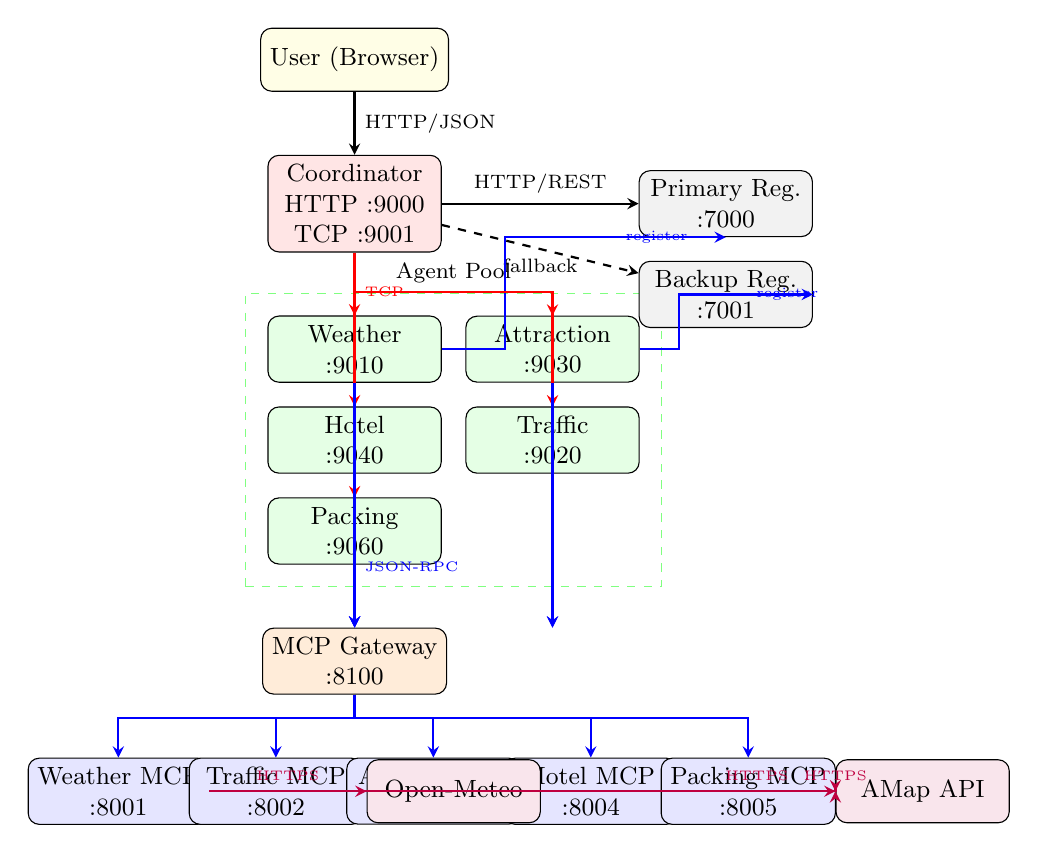
\begin{tikzpicture}[
    node distance=1.2cm,
    box/.style={rectangle, draw, rounded corners, minimum width=2.2cm, minimum height=0.8cm, align=center, font=\small},
    server/.style={box, fill=blue!10},
    agent/.style={box, fill=green!10},
    gateway/.style={box, fill=orange!15},
    coord/.style={box, fill=red!10},
    reg/.style={box, fill=gray!10},
    user/.style={box, fill=yellow!10},
    arrow/.style={->, >=stealth, thick},
]

% User
\node[user] (user) {User (Browser)};

% Coordinator
\node[coord, below=0.8cm of user] (coord) {Coordinator\\HTTP :9000\\TCP :9001};

% Registry
\node[reg, right=2.5cm of coord] (reg1) {Primary Reg.\\:7000};
\node[reg, below=0.3cm of reg1] (reg2) {Backup Reg.\\:7001};

% Agent Pool
\node[agent, below=0.8cm of coord] (weather_a) {Weather\\:9010};
\node[agent, right=0.3cm of weather_a] (attract_a) {Attraction\\:9030};
\node[agent, below=0.3cm of weather_a] (hotel_a) {Hotel\\:9040};
\node[agent, right=0.3cm of hotel_a] (traffic_a) {Traffic\\:9020};
\node[agent, below=0.3cm of hotel_a] (pack_a) {Packing\\:9060};

% Agent Pool boundary
\begin{scope}[on background layer]
\node[fit=(weather_a)(attract_a)(traffic_a)(pack_a), draw=green!50, dashed, inner sep=8pt, label={[font=\footnotesize]above:Agent Pool}] {};
\end{scope}

% Gateway
\node[gateway, below=0.8cm of pack_a] (gw) {MCP Gateway\\:8100};

% MCP Servers
\node[server, below=0.8cm of gw, xshift=-3cm] (weather_m) {Weather MCP\\:8001};
\node[server, below=0.8cm of gw, xshift=-1cm] (traffic_m) {Traffic MCP\\:8002};
\node[server, below=0.8cm of gw, xshift=1cm] (attract_m) {Attract MCP\\:8003};
\node[server, below=0.8cm of gw, xshift=3cm] (hotel_m) {Hotel MCP\\:8004};
\node[server, below=0.8cm of gw, xshift=5cm] (pack_m) {Packing MCP\\:8005};

% External APIs
\node[box, fill=purple!10, right=2cm of hotel_m] (amap) {AMap API};
\node[box, fill=purple!10, right=2cm of weather_m] (meteo) {Open-Meteo};

% Arrows: User -> Coordinator
\draw[arrow] (user) -- (coord) node[midway, right, font=\scriptsize] {HTTP/JSON};

% Coordinator -> Registry
\draw[arrow] (coord) -- (reg1) node[midway, above, font=\scriptsize] {HTTP/REST};
\draw[arrow, dashed] (coord) -- (reg2) node[midway, below, font=\scriptsize] {fallback};

% Registry <- Agent (register)
\draw[arrow, blue] (weather_a.east) -- ++(0.8,0) |- (reg1.south) node[near end, right, font=\tiny, blue] {register};
\draw[arrow, blue] (attract_a.east) -- ++(0.5,0) |- (reg2.east) node[near end, right, font=\tiny, blue] {register};

% Coordinator -> Agent (TCP A2A)
\draw[arrow, red] (coord.south) -- ++(0,-0.5) -| (weather_a.north) node[near start, right, font=\tiny, red] {TCP};
\draw[arrow, red] (coord.south) -- ++(0,-0.5) -| (attract_a.north);
\draw[arrow, red] (coord.south) -- ++(0,-0.5) -| (hotel_a.north);
\draw[arrow, red] (coord.south) -- ++(0,-0.5) -| (traffic_a.north);
\draw[arrow, red] (coord.south) -- ++(0,-0.5) -| (pack_a.north);

% Agent -> Gateway (JSON-RPC)
\draw[arrow, blue] (weather_a.south) -- (weather_a.south |- gw.north) node[near end, right, font=\tiny, blue] {JSON-RPC};
\draw[arrow, blue] (attract_a.south) -- (attract_a.south |- gw.north);
\draw[arrow, blue] (hotel_a.south) -- (hotel_a.south |- gw.north);
\draw[arrow, blue] (traffic_a.south) -- (traffic_a.south |- gw.north);
\draw[arrow, blue] (pack_a.south) -- (pack_a.south |- gw.north);

% Gateway -> MCP
\draw[arrow, blue] (gw.south) -- ++(0,-0.3) -| (weather_m.north);
\draw[arrow, blue] (gw.south) -- ++(0,-0.3) -| (traffic_m.north);
\draw[arrow, blue] (gw.south) -- ++(0,-0.3) -| (attract_m.north);
\draw[arrow, blue] (gw.south) -- ++(0,-0.3) -| (hotel_m.north);
\draw[arrow, blue] (gw.south) -- ++(0,-0.3) -| (pack_m.north);

% MCP -> External APIs
\draw[arrow, purple] (weather_m.east) -- (meteo.west) node[midway, above, font=\tiny, purple] {HTTPS};
\draw[arrow, purple] (attract_m.east) -- (attract_m.east -| amap.west) -- (amap.west) node[midway, above, font=\tiny, purple] {HTTPS};
\draw[arrow, purple] (hotel_m.east) -- (amap.west) node[midway, above, font=\tiny, purple] {HTTPS};
\draw[arrow, purple] (traffic_m.east) -- (traffic_m.east -| amap.west) -- (amap.west);

\end{tikzpicture}
\end{document}
